\subsection{Logistical: Model of Reverse Logistic for the compilation of plastic to recycling for the Impression 3D in the context of a Fab Lab}

Concerning the logistical aspect, figure \ref{Context.Pavlo} shows the consideration for the developing of the logistical elements.
The work developed by Pavlo Santander were focalised to analyze the feasibility of using a Fab Lab as a plastic recycling point for 3D impression considering its context and resources.
Therefore, a logistic model to collect the plastic for the FabLab was studied.
Processes such as \textit{sorting, cleaning, additives, pigments} were not considered in the model
Moreover, only schools and collegues were considered. 

\begin{figure}[H]
	\centering
	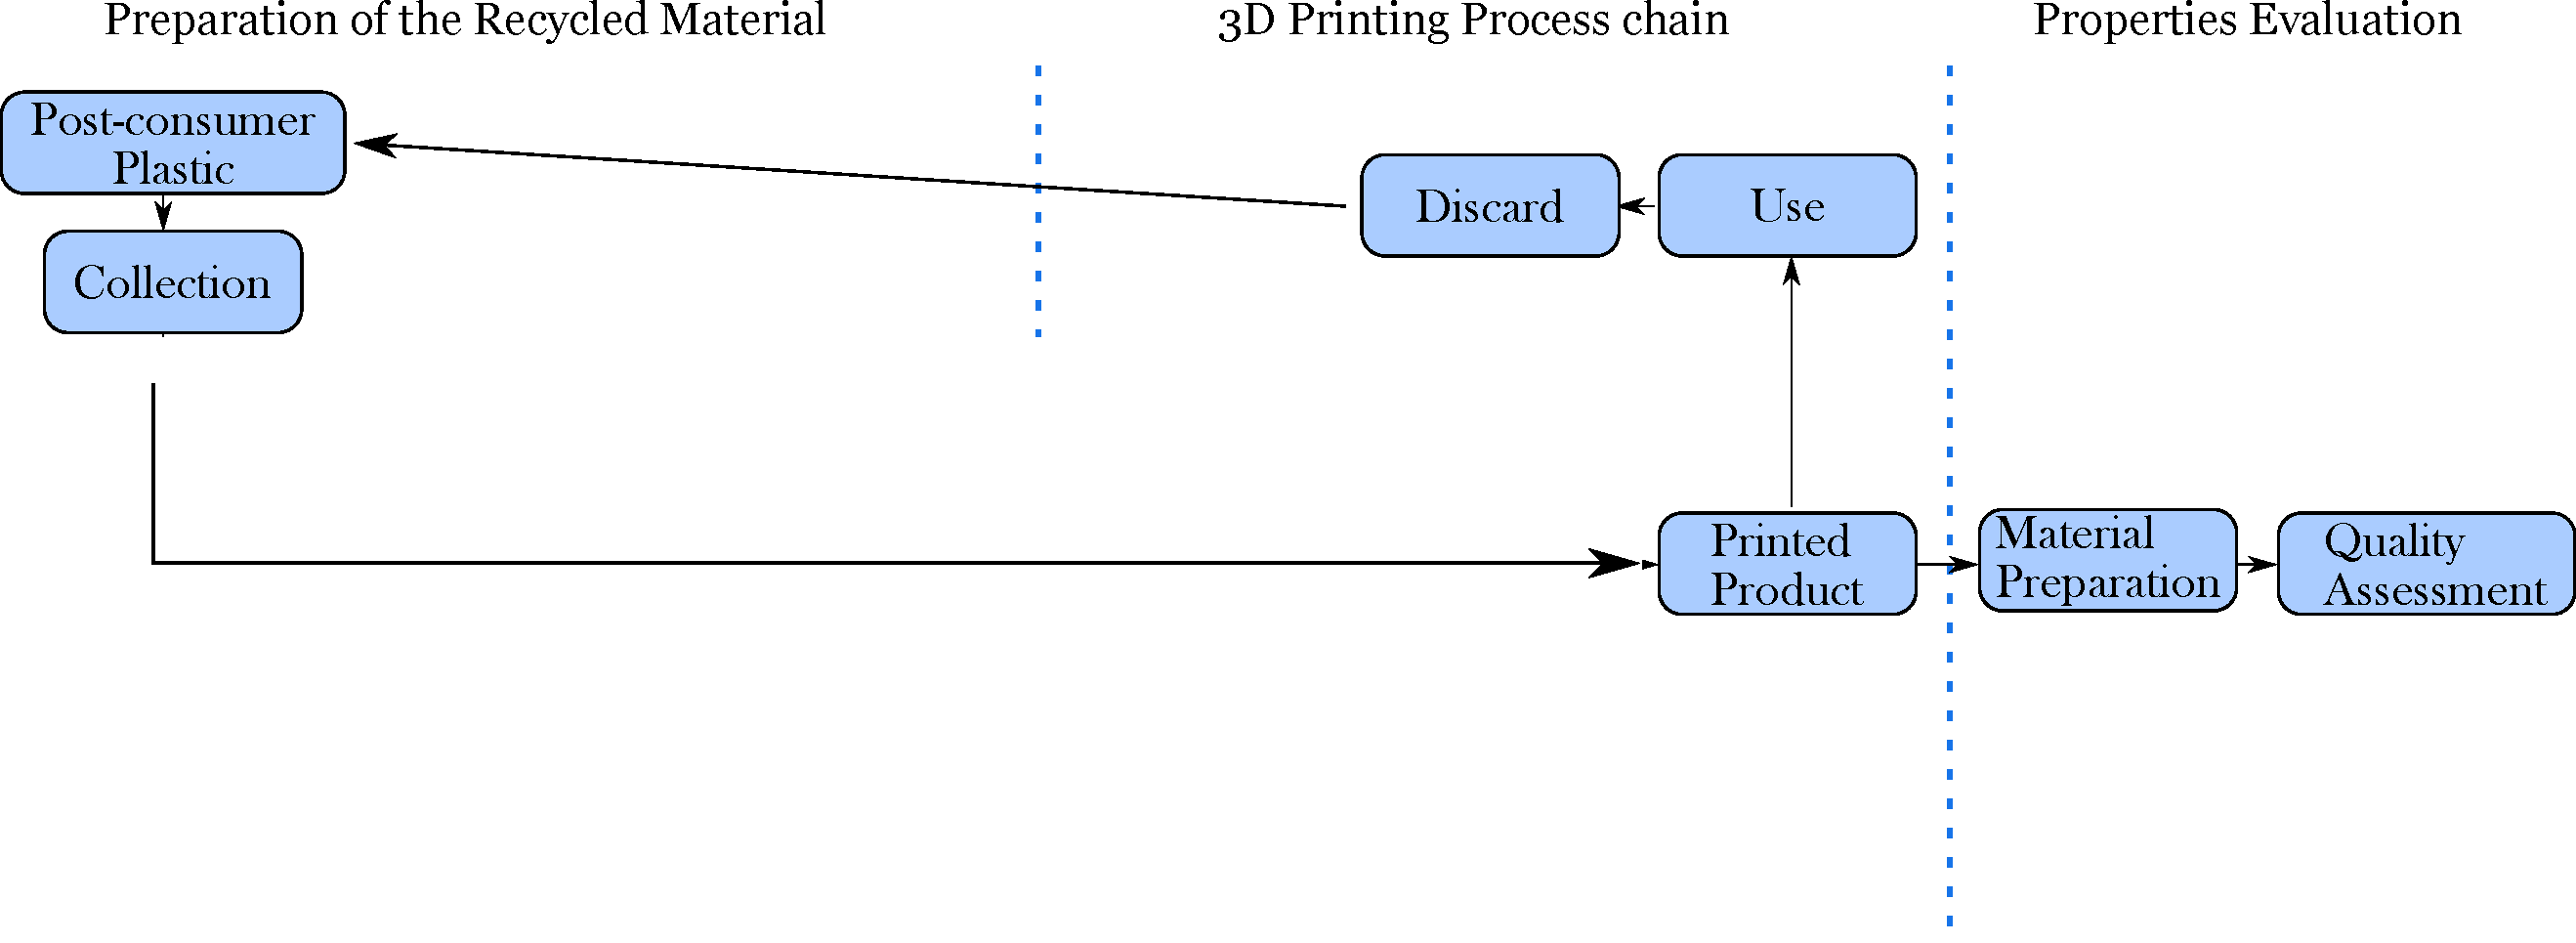
\includegraphics[width=0.7\textwidth]{Figures/Pavlo/Context-Pavlo.pdf}
	\caption{Previous results from the logistic model.}
	\label{Context.Pavlo}		
\end{figure}



The main goals of the mathematical model were:


\begin{itemize}[noitemsep]
	\item Quantity of plastic to recycle
	\item Select best collecting points from potential sources
	\item Establish optimal routes
	\item Comparation of means of transport
	\item Economical and enviromental aspects
\end{itemize}

The objective function (OF) of the mathematical model is represented as a benefit to maximizing. 
In the context of a Fab Lab, the benefit is represented of two points of view: Operational and Environmental. 

\begin{align*} 
OF &= Max[Benefice] \\ 
OF &=  Max[\textcolor{Orange}{Operational~Benefice~(OB)} + \textcolor{Purple}{Environmental~Benefice~(EB) }]  \\
\textcolor{Orange}{OB} &=  \textcolor{RoyalBlue}{Cost~Virgin} - \textcolor{SkyBlue}{Recycling~Cost} \\
\textcolor{Purple}{EB} &= \textcolor{ForestGreen}{Emissions~CO_{2}(Virgin)} - \textcolor{LimeGreen}{Emissions~CO_{2}(Recycling)}
\end{align*}




\begin{figure}[H]
	\centering
		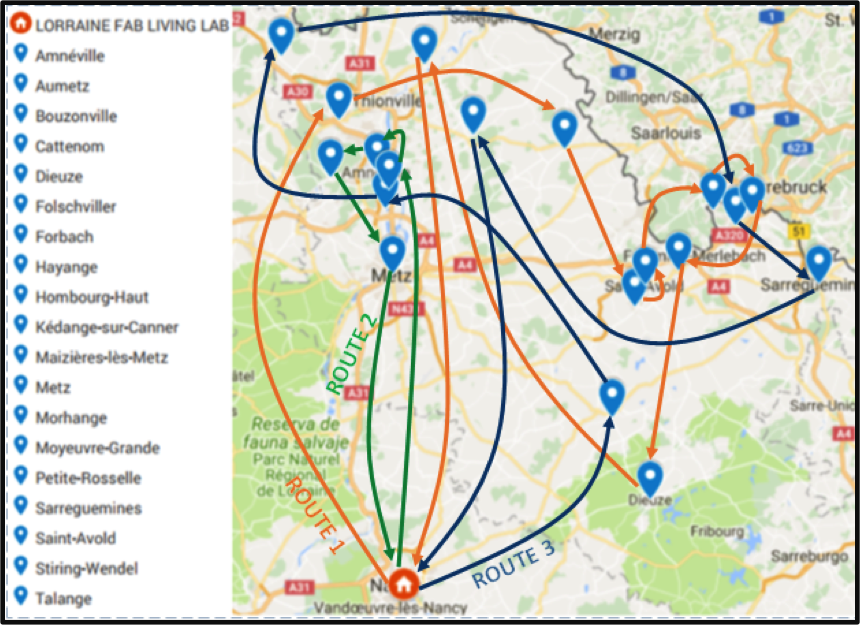
\includegraphics[width=0.7\textwidth]{Figures/Pavlo/Results.png}
		\caption{Previous results from the logistic model.}
		\label{Results.Pavlo}		
\end{figure}

